\documentclass[a4paper]{article}
\usepackage[affil-it]{authblk}
%\usepackage[backend=bibtex,style=numeric]{biblatex}
\usepackage{graphicx} % Required for inserting images
\usepackage{caption}

\usepackage{ctex}
\usepackage{epstopdf}
\usepackage{amsfonts,amssymb}
\usepackage{tikz}
\usetikzlibrary{chains}
\usepackage{listings}
\usepackage{xcolor}
\usepackage{float}
\usepackage{hyperref}
\usepackage{bookmark}
\usepackage{subfig}
\usepackage{listings,matlab-prettifier} % MATLAB 美化包
% \lstset{
%         style=Matlab-editor,
%         numbers      = left,
%         frame        = single,
% }
\usepackage{amsmath}
\usepackage{chngcntr}
\counterwithout{equation}{section}
\counterwithout{figure}{section}

\usepackage{geometry}
\geometry{margin=1.5cm, vmargin={0pt,1cm}}
\setlength{\topmargin}{-1cm}
\setlength{\paperheight}{29.7cm}
\setlength{\textheight}{25.3cm}


\begin{document}
% =================================================
\title{NA Theoretical homework \#3}

\author{陈澎 Chen Peng 3220103443
  \thanks{Email: \texttt{cpzju@zju.edu.cn}}}
\affil{Xinji 2201, Zhejiang University }


\date{\today}

\maketitle

% ============================================
\section*{I.}
Set $q(x)=(2-x)^3$. Since $s\in \mathbb{S}_3^2$, it induces that $p(1)=q(1)=1$, $p'(1)=q'(1)=-3$, $p''(1)=q''(1)=6$. Besides $p(0)=s(0)=0$.
Construct the divided table.

\begin{table}[!htbp]
  \centering
  \begin{tabular}{c|cccc}
    0 & 0 & & & \\
    1 & 1 & 1 & &  \\
    1 & 1 &-3 & -4 & \\
    1 & 1 &-3 & 3 & 7 \\
  \end{tabular}
\end{table}

So $p(x)=x-4x(x-1)+7x(x-1)^2$, i.e.
$$p(x)=7x^3-18x^2+12x.$$

it induces that $p''(x)=42x-36$. Then $p''(0)=-36\neq0$. So it is not a natural cubic spline.

\section*{II.}
\subsection*{II-a.}
From theorem 3.14, the set of splines $\mathbb{S}_2^1(x_1,x_2,\ldots,x_n)$ is a linear space with dimension n+1. 
However, there are only n nonlinear related conditions. So an additional condition needed to determine $s$ uniquel

\subsection*{II-b.}
Construct the divided table. Set $K_i=\dfrac{f_{i+1}-f_i}{x_{i+1}-x_i}$.

\begin{table}[!htbp]
  \centering
  \begin{tabular}{c|ccc}
    $x_i$ & $f_i$ & &  \\
    $x_i$ & $f_i$ & $m_i$ &   \\
    $x_{i+1}$ & $f_{i+1}$ & $K_i$ & $\dfrac{K_i-m_i}{x_{i+1}-x_i}$  \\
  \end{tabular}
\end{table}

So, for $i=1,2,\ldots,n-1$, 
$$p_{i}(x)=f_i+m_i(x-x_i)+\dfrac{K_i-m_i}{x_{i+1}-x_i}(x-x_i)^2,\ x\in[x_i,x_{i+1}].$$

\subsection*{II-c.}
From(b), $s\in C^1$ implies that $p'_{i}(x_{i+1})=p'_{i+1}(x_{i+1})$, i.e. 
$$m_i+2\dfrac{K_i-m_i}{x_{i+1}-x_i}(x_{i+1}-x_i) = m_{i+1}+2\dfrac{K_{i+1}-m_{i+1}}{x_{i+2}-x_{i+1}}(x_{i+1}-x_{i+1}).$$

Simplifying it, we have
$$m_{i+1}=2K_i-m_i,$$
for $i=1,2,\ldots,n-1$.

$K_i$ can be computed and $m_1$ is given. Thus $m_{2},m_{2},\ldots,m_{n-1}$ can be computed by using the above equation.

\section*{III.}
From the definition of natural cubic spline, we have
$$
  \left\{\begin{aligned}
    s_2(0)&=s_1(0)=1+c; \\
    s'_2(0)&=s'_1(0)=3c; \\
    s''_2(0)&=s''_1(0)=6c; 
  \end{aligned}
  \right.
$$

Set $s_2(1)=s(1)=a$.

Construct the divided table.

\begin{table}[!htbp]
  \centering
  \begin{tabular}{c|cccc}
    
    0 & $1+c$ & & & \\
    0 & $1+c$ & $3c$ & &  \\
    0 & $1+c$ & $3c$ & $3c$ & \\
    1 & $a$ &$a-1-c$ & $a-1-4c$ & $a-1-7c$ \\
  \end{tabular}
\end{table}


So $$s_2(x)=1+c+3cx+3cx^2-(1+7c-a)x^3.$$

From definition 3.5, the natural cubic spline s satisfies 
$$s''_1(-1)=s''_2(1)=0.$$

Since $s''_2(x)=6c-6(1+7c-a)x$, we can induce that $a=6c+1$.

So $$s_2(x)=1+c+3cx+3cx^2-cx^3.$$

When $a=-1$, we can induces that $c=-\frac{1}{3}$.

\section*{IV.}
\subsection*{IV-a.}
Set 
$$
s(x)=\left\{
\begin{aligned}
  &p_1(x), &x\in [-1,0);\\
  &p_2(x), &x\in [0,1].
\end{aligned}
\right.
$$

For $p_1(x)$, we have $p_1(-1)=f(-1)$, $p_1(0)=f(0)$, $p''_1(-1)=0$. Set $p'_1(-1)=m_1$. Construct the divided table.

\begin{table}[H]
  \centering
  \begin{tabular}{c|cccc}
    -1 & 0 & & & \\
    -1 & 0 & $m_1$ & &  \\
    -1 & 0 & $m_1$ & 0 & \\
    0 & 1 & 1 & $1-m_1$ & $1-m_1$ \\
  \end{tabular}
\end{table}

So $$p_1(x)=m_1(x+1)+(1-m_1)(x+1)^3.$$

For $p_2(x)$, we have $p_2(0)=f(0)$, $p_2(1)=f(1)$, $p''_2(1)=0$. Set $p'_2(1)=m_2$. Construct the divided table.

\begin{table}[H]
  \centering
  \begin{tabular}{c|cccc}
    0 & 1 & & & \\
    0 & 0 & -1 & &  \\
    0 & 0 & $m_2$ & $m_2+1$ & \\
    1 & 0 & $m_2$ & 0 & $-m_2-1$ \\
  \end{tabular}
\end{table}

So $$p_2(x)=1-x+(m_2+1)x(x-1)-(m_2+1)x(x-1)^2.$$

From the definition of natural cubic spline, it induces that $p'_2(0)=p'_1(0)$, $p''_2(0)=p''_1(0)$, i.e.
$$
\left\{
\begin{aligned}
  &m_1+3(1-m_1)=-1-(m_2+1)-(m_2+1);\\
  &6(1-m_1)=2(m_2+1)+4(m_2+1).
\end{aligned}
\right.
$$

Solve the equations. We have 
$$
\left\{
\begin{aligned}
  &m_1=\frac{3}{2};\\
  &m_2=-\frac{3}{2}.
\end{aligned}
\right.
$$

So $p_1(x)=\frac{3}{2}(x+1)-\frac{1}{2}(x+1)^3$ and $p_2(x)=1-x-\frac{1}{2}x(x-1)+\frac{1}{2}x(x-1)^2$.

Thus
$$
s(x)=
\left\{
\begin{aligned}
  &-\frac{1}{2}x^3-\frac{3}{2}x^2+1, &x\in [-1,0);\\
  &\frac{1}{2}x^3-\frac{3}{2}x^2+1, &x\in [0,1].
\end{aligned}
\right.
$$

\subsection*{IV-b.}
$$
s''(x)=
\left\{
\begin{aligned}
  &-3(x+1), &x\in [-1,0);\\
  &3(x-1), &x\in [0,1].
\end{aligned}
\right.
$$

So 
$$
\int_{-1}^{1}[s''(x)]^2 \mathrm{d}x=6.
$$

\subsubsection*{(i)}
Set $s_1(x)$.

We have $s_1(-1)=f(-1)$, $s_1(0)=f(0)$ and $s_1(1)=f(1)$. Construct the divided table.

\begin{table}[H]
  \centering
  \begin{tabular}{c|ccc}
    -1 & 0 & &  \\
    0 & 1 & 1 &   \\
    1 & 0 & -1 & -1  \\
  \end{tabular}
\end{table}

So $p_3(x)=x+1-(x+1)x=1-x^2$.

Thus 
$$
s''_1(x)=-2.
$$

We have 
$$
\int_{-1}^{1}[s''_1(x)]^2 \mathrm{d}x=8>6.
$$

Therefore, the bending energy of $s_1(x)$ is more than $s(x)$.

\subsubsection*{(ii)}
It can be computed that $$f''(x)=-\frac{\pi^2}{4}\cos(\frac{\pi}{2}x).$$

So $$\int_{-1}^{1}[f''(x)]^2 \mathrm{d}x=\frac{\pi^4}{16}\approx6.088>6.$$

Therefore, the bending energy of $f(x)$ is more than $s(x)$.

\section*{V.}
\subsection*{V-a.}
From Definition 3.21 and Example 3.24, we have
$$
B^1_i(x)=\hat{B}_i(x)=
\left\{
\begin{aligned}
  &\frac{x-t_{i-1}}{t_i-t_{i-1}}, &x\in (t_{i-1},t_i];\\
  &\frac{t_{i+1}-x}{t_{i+1}-t_{i}}, &x\in (t_i,t_{i+1}]; \\
  &0, &\text{otherwise}.
\end{aligned}
\right.
$$

From Definition 3.23, we have 
$$B_i^{2}(x)=\frac{x-t_{i-1}}{t_{i+1}-t_{i-1}}B_i^1(x)+\frac{t_{i+2}-x}{t_{i+2}-t_i}B_{i+1}^1(x).$$

When $x\in(t_{i-1},t_i]$, $B_i(x)=\dfrac{x-t_{i-1}}{t_i-t_{i-1}}$ and $B_{i+1}(x)=0$.

When $x\in (t_i,t_{i+1}]$, $B_i(x)=\dfrac{t_{i+1}-x}{t_{i+1}-t_{i}}$, and $B_{i+1}(x)=\dfrac{x-t_{i}}{t_{i+1}-t_{i}}$.

When $x\in(t_{i-1},t_i]$, $B_i(x)=0$ and $B_{i+1}(x)=\dfrac{t_{i+2}-x}{t_{i+2}-t_{i+1}}$.

So 
$$
B_i^2(x)=\begin{cases}
  \dfrac{(x-t_{i-1})^2}{(t_{i+1}-t_{i-1})(t_i-t_{i-1})},&x\in(t_{i-1},t_i];\\
  \dfrac{(x-t_{i-1})(t_{i+1}-x)}{(t_{i+1}-t_{i-1})(t_{i+1}-t_i)}+\dfrac{(t_{i+2}-x)(x-t_i)}{(t_{i+2}-t_i)(t_{i+1}-t_i)},&x\in(t_i,t_{i+1}];\\
  \dfrac{(t_{i+2}-x)^2}{(t_{i+2}-t_i)(t_{i+2}-t_{i+1})},&x\in(t_{i+1},t_{i+2}];\\
  0,&\text{otherwise.}
\end{cases}
$$


\subsection*{V-b.}
$$
\frac{\mathrm{d}}{\mathrm{d}x}B_i^2(x)=\begin{cases}
  \dfrac{2(x-t_{i-1})}{(t_{i+1}-t_{i-1})(t_i-t_{i-1})},&x\in(t_{i-1},t_i];\\
  \dfrac{-2x+t_{i-1}+t_{i+1}}{(t_{i+1}-t_{i-1})(t_{i+1}-t_i)}+\dfrac{-2x+t_{i+2}+t_i}{(t_{i+2}-t_i)(t_{i+1}-t_i)},&x\in(t_i,t_{i+1}];\\
  \dfrac{2(x-t_{i+2})}{(t_{i+2}-t_i)(t_{i+2}-t_{i+1})},&x\in(t_{i+1},t_{i+2}];\\
  0,&\text{otherwise.}
\end{cases}
$$

It can be calculated that $\frac{\mathrm{d}}{\mathrm{d}x}B_i^2(t_i)=\dfrac{2}{t_{i+1}-t_{i-1}}$. Since
$$
\begin{aligned}
  \lim_{x\rightarrow t_{i}^+} \frac{\mathrm{d}}{\mathrm{d}x}B_i^2(x)&=\dfrac{t_{i-1}+t_{i+1}-2t_i}{(t_{i+1}-t_{i-1})(t_{i+1}-t_i)}+\dfrac{1}{t_{i+1}-t_i}\\
  &=\dfrac{2t_{i+1}-2t_i}{(t_{i+1}-t_{i-1})(t_{i+1}-t_i)}\\
  &=\dfrac{2}{t_{i+1}-t_{i-1}},
\end{aligned}
$$
so $\frac{\mathrm{d}}{\mathrm{d}x}B_i^2(x)$ is continuous at $t_i$.

It can be calculated that $\frac{\mathrm{d}}{\mathrm{d}x}B_i^2(t_{i+1})=-\dfrac{2}{t_{i+2}-t_{i}}$. Since
$$
\begin{aligned}
  \lim_{x\rightarrow t_{i+1}^+} \frac{\mathrm{d}}{\mathrm{d}x}B_i^2(x)&=\dfrac{(t_{i+1}-t_{i+2})}{(t_{i+2}-t_{i})(t_{i+2}-t_{i+1})}\\
  &=-\dfrac{2}{t_{i+2}-t_{i}},
\end{aligned}
$$
$\frac{\mathrm{d}}{\mathrm{d}x}B_i^2(x)$ is continuous at $t_{i+1}$.

\subsection*{V-c.}
$$
\frac{\mathrm{d}}{\mathrm{d}x}B_i^2(x)=\begin{cases}
  \dfrac{2(x-t_{i-1})}{(t_{i+1}-t_{i-1})(t_i-t_{i-1})},&x\in(t_{i-1},t_i];\\
  \dfrac{-2x+t_{i-1}+t_{i+1}}{(t_{i+1}-t_{i-1})(t_{i+1}-t_i)}+\dfrac{-2x+t_{i+2}+t_i}{(t_{i+2}-t_i)(t_{i+1}-t_i)},&x\in(t_i,t_{i+1}];\\
  \dfrac{2(x-t_{i+2})}{(t_{i+2}-t_i)(t_{i+2}-t_{i+1})},&x\in(t_{i+1},t_{i+2}];\\
  0,&\text{otherwise.}
\end{cases}
$$

When $x\in (t_{i-1},t_{i}]$, $\frac{\mathrm{d}}{\mathrm{d}x}B_i^2(x)>0$.

When $x\in (t_{i},t_{i+1}]$, $\frac{\mathrm{d}}{\mathrm{d}x}B_i^2(x)$ is monotonically decreasing. Since $\frac{\mathrm{d}}{\mathrm{d}x}B_i^2(t_i)>0$ and $\frac{\mathrm{d}}{\mathrm{d}x}B_i^2(t_{i+1})<0$, 
there exists only one $x^{*}\in (t_{i},t_{i+1}]$ satisfies $\frac{\mathrm{d}}{\mathrm{d}x}B_i^2(x^{*})=0$. After simplifying, we have 
$$
x^{*}=\dfrac{t_{i+2}t_{i+1}-t_{i}t_{i-1}}{t_{i+2}+t_{i+1}-t_{i}-t_{i-1}}.
$$

\subsection*{V-d.}
When $x\in (t_{i-1},t_{i}]$, $\frac{\mathrm{d}}{\mathrm{d}x}B_i^2(x)$ is monotonically increasing. So 
$$0=\frac{\mathrm{d}}{\mathrm{d}x}B_i^2(t_{i-1})<\frac{\mathrm{d}}{\mathrm{d}x}B_i^2(x)\leq \frac{\mathrm{d}}{\mathrm{d}x}B_i^2(t_i)=\dfrac{t_i-t_{i-1}}{t_{i+1}-t_{i-1}}<1.$$

When $x\in (t_{i},t_{i+1}]$, $\frac{\mathrm{d}}{\mathrm{d}x}B_i^2(x)$ is monotonically increasing at $(t_i,x^{*})$ and monotonically decreasing at $[x^{*},t_{i+1}]$. So 
$$\frac{\mathrm{d}}{\mathrm{d}x}B_i^2(x)>\min\{\frac{\mathrm{d}}{\mathrm{d}x}B_i^2(t_{i}),\frac{\mathrm{d}}{\mathrm{d}x}B_i^2(t_{i+1})\}>0,$$
and 
$$
\begin{aligned}
  \frac{\mathrm{d}}{\mathrm{d}x}B_i^2(x)_{\mathrm{max}}&=\frac{\mathrm{d}}{\mathrm{d}x}B_i^2(x^{*})\\
  &<\dfrac{t_{i+1}-x^{*}}{t_{i+1}-t_{i}}+\dfrac{(t_{i+2}-x^{*})(x^{*}-t_i)}{(t_{i+2}-t_i)(t_{i+1}-t_i)}\\
  &=\dfrac{(t_{i+1}-x^{*})(t_{i+2}-t_i)+(t_{i+2}-x^{*})(x^{*}-t_i)}{(t_{i+2}-t_i)(t_{i+1}-t_i)}\\
  &=\dfrac{-x^{*^2}+2t_{i}x^{*}+t_{i+1}t_{i+2}-t_{i}t_{i+1}-t_{i+2}t_{i}}{(t_{i+2}-t_i)(t_{i+1}-t_i)}\\
  &\leq\dfrac{-t_{i}^2+2t_{i}^2+t_{i+1}t_{i+2}-t_{i}t_{i+1}-t_{i+2}t_{i}}{(t_{i+2}-t_i)(t_{i+1}-t_i)}\\
  &=1,
\end{aligned}
$$
i.e. $0<\frac{\mathrm{d}}{\mathrm{d}x}B_i^2(x)<1$, for $x\in(t_{i},t_{i+1}]$.

When $x\in (t_{i+1},t_{i+2}]$, $\frac{\mathrm{d}}{\mathrm{d}x}B_i^2(x)$ is monotonically decreasing at $(t_{i+1},t_{i+2}]$. So 
$$
0<\frac{\mathrm{d}}{\mathrm{d}x}B_i^2(t_{i+2})<\frac{\mathrm{d}}{\mathrm{d}x}B_i^2(x)\leq \frac{\mathrm{d}}{\mathrm{d}x}B_i^2(t_{i+2})<1.
$$

When $x$ doesn't satisfies the above condition, $\frac{\mathrm{d}}{\mathrm{d}x}B_i^2(x)=0$.

In conclusion, $\frac{\mathrm{d}}{\mathrm{d}x}B_i^2(x)\in[0,1)$.


\subsection*{V-e.}
The image is shown in Fig.\ref{fig1}.

\begin{figure}[H]
  \centering
  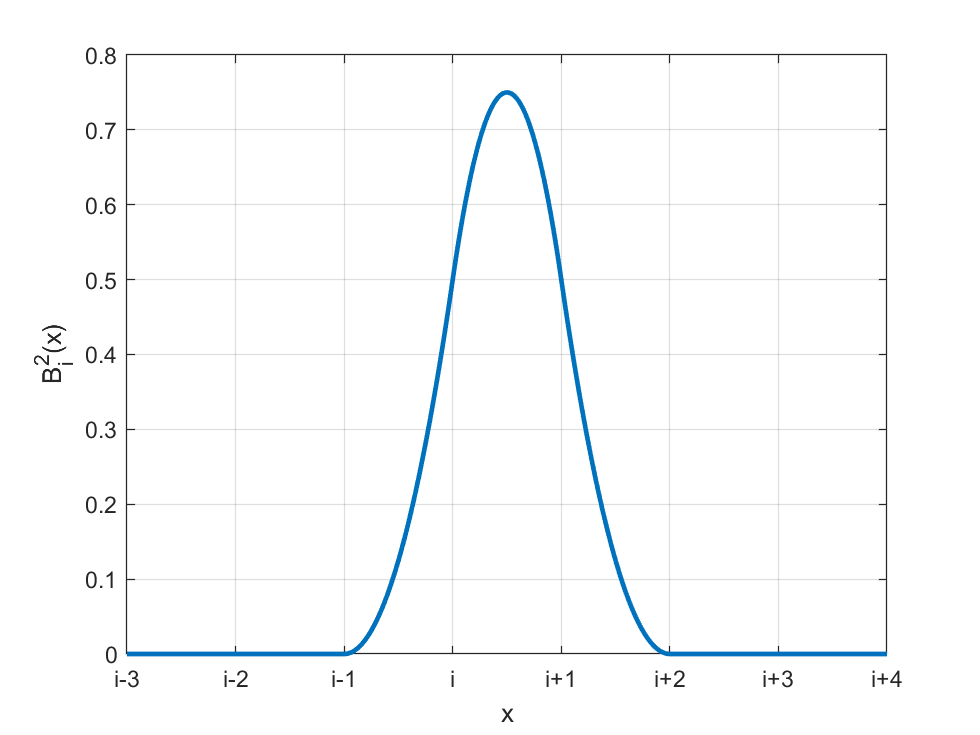
\includegraphics[width=0.6\textwidth]{./images/B_i^2.png}
  \renewcommand{\figurename}{Fig.}
  \caption{B-spline $B^2_i(x)$ for $t_j = j$}
  \label{fig1}
\end{figure}

\section*{VI.}
We know that 
$$
B_i^2(x)=\begin{cases}
  \dfrac{(x-t_{i-1})^2}{(t_{i+1}-t_{i-1})(t_i-t_{i-1})},&x\in(t_{i-1},t_i];\\
  \dfrac{(x-t_{i-1})(t_{i+1}-x)}{(t_{i+1}-t_{i-1})(t_{i+1}-t_i)}+\dfrac{(t_{i+2}-x)(x-t_i)}{(t_{i+2}-t_i)(t_{i+1}-t_i)},&x\in(t_i,t_{i+1}];\\
  \dfrac{(t_{i+2}-x)^2}{(t_{i+2}-t_i)(t_{i+2}-t_{i+1})},&x\in(t_{i+1},t_{i+2}];\\
  0,&\text{otherwise.}
\end{cases}
$$

As for left hand side of the equation, 
$$
\begin{aligned}
  &(t_{i+2}-t_{i-1})[t_{i-1},t_{i},t_{i+1},t_{i+2}](t-x)_{+}^{2}\\
  =&[t_{i},t_{i+1},t_{i+2}](t-x)_{+}^{2}-[t_{i-1},t_{i},t_{i+1}](t-x)_{+}^{2}\\
  =&\dfrac{[t_{i+1},t_{i+2}](t-x)_{+}^{2}-[t_{i},t_{i+1}](t-x)_{+}^{2}}{t_{i+2}-t_{i}}-\dfrac{[t_{i},t_{i+1}](t-x)_{+}^{2}-[t_{i-1},t_{i}](t-x)_{+}^{2}}{t_{i+1}-t_{i-1}}\\
  =&\dfrac{(t_{i+2}-x)_{+}^{2}-(t_{i+1}-x)_{+}^{2}}{(t_{i+2}-t_{i})(t_{i+2}-t_{i+1})}-\dfrac{(t_{i+1}-x)_{+}^{2}-(t_{i}-x)_{+}^{2}}{(t_{i+2}-t_{i})(t_{i+1}-t_{i})}-\dfrac{(t_{i+1}-x)_{+}^{2}-(t_{i}-x)_{+}^{2}}{(t_{i+1}-t_{i-1})(t_{i+1}-t_{i})}+\dfrac{(t_{i}-x)_{+}^{2}-(t_{i-1}-x)_{+}^{2}}{(t_{i+1}-t_{i-1})(t_{i}-t_{i-1})}.
\end{aligned}
$$

When $x\in (t_{i-1},t_{i}]$, 
$$
\begin{aligned}
  \text{LHS}&=\dfrac{t_{i+2}+t_{i+1}-2x}{t_{i+2}-t_{i}}-\dfrac{t_{i+1}+t_{i}-2x}{t_{i+2}-t_{i}}-\dfrac{t_{i+1}+t_{i}-2x}{t_{i+1}-t_{i-1}}+\dfrac{(t_{i}-x)^{2}}{(t_{i+1}-t_{i-1})(t_{i}-t_{i-1})}\\
  &=\dfrac{2x-t_{i}+t_{i-1}}{t_{i+1}-t_{i-1}}+\dfrac{(t_{i}-x)^{2}}{(t_{i+1}-t_{i-1})(t_{i}-t_{i-1})}\\
  &=\dfrac{(x-t_{i-1})^2}{(t_{i+1}-t_{i-1})(t_i-t_{i-1})}.
\end{aligned}
$$

When $x\in (t_{i},t_{i+1}]$, 
$$
\begin{aligned}
  \text{LHS}&=\dfrac{t_{i+2}+t_{i+1}-2x}{t_{i+2}-t_{i}}-\dfrac{(t_{i+1}-x)^{2}}{(t_{i+2}-t_{i})(t_{i+1}-t_{i})}-\dfrac{(t_{i+1}-x)^{2}}{(t_{i+1}-t_{i-1})(t_{i+1}-t_{i})}\\
  &=\dfrac{-x^2+2t_{i}x+t_{i+2}(t_{i+1}-t_{i})-t_{i+1}t_i}{(t_{i+2}-t_i)(t_{i+1}-t_i)}+\dfrac{(x-t_{i-1})(t_{i+1}-x)+(t_{i+1}-t_{i-1})x+t_{i-1}t_{i+1}-t_{i+1}^2}{(t_{i+1}-t_{i-1})(t_{i+1}-t_i)}\\
  &=\dfrac{-x^2+2t_{i}x+t_{i+2}(t_{i+1}-t_{i})-t_{i+1}t_i}{(t_{i+2}-t_i)(t_{i+1}-t_i)}+\dfrac{x-t_{i+1}}{t_{i+1}-t_i}+\dfrac{(x-t_{i-1})(t_{i+1}-x)}{(t_{i+1}-t_{i-1})(t_{i+1}-t_i)}\\
  &=\dfrac{(x-t_{i-1})(t_{i+1}-x)}{(t_{i+1}-t_{i-1})(t_{i+1}-t_i)}+\dfrac{(t_{i+2}-x)(x-t_i)}{(t_{i+2}-t_i)(t_{i+1}-t_i)}.
\end{aligned}
$$

When $x\in (t_{i+1},t_{i+2}]$, 
$$
\begin{aligned}
  \text{LHS}&=\dfrac{(t_{i+2}-x)^{2}}{(t_{i+2}-t_{i})(t_{i+2}-t_{i+1})}.
\end{aligned}
$$

When $x\leq t_{i-1}$, 
$$
\begin{aligned}
  \text{LHS}&=(\dfrac{t_{i+2}+t_{i+1}-2x}{t_{i+2}-t_{i}}-\dfrac{t_{i+1}+t_{i}-2x}{t_{i+2}-t_{i}})-(\dfrac{t_{i+1}+t_{i}-2x}{t_{i+1}-t_{i-1}}-\dfrac{t_{i}+t_{i-1}-2x}{t_{i+1}-t_{i-1}})\\
  &=1-1\\
  &=0.
\end{aligned}
$$

When $x>t_{i+2}$, $\text{LHS}=0$.

So the equation holds.

\section*{VII.}
From theorem 3.34, we know that 
$$
\frac{\mathrm{d}}{\mathrm{d}x}B_i^n(x)=\frac{nB_i^{n-1}(x)}{t_{i+n-1}-t_{i-1}}-\frac{nB_{i+1}^{n-1}(x)}{t_{i+n}-t_i}.
$$

Integral each side from $t_{i-1}$ to $t_{i+n}$. It induces that 
$$
\int_{t_{i-1}}^{t_{i+n}}\frac{\mathrm{d}}{\mathrm{d}x}B_i^n(x)\mathrm{d}x=\int_{t_{i-1}}^{t_{i+n}}(\frac{nB_{i}^{n-1}(x)}{t_{i+n-1}-t_{i-1}}-\frac{nB_{i+1}^{n-1}(x)}{t_{i+n}-t_{i}})\mathrm{d}x,
$$
i.e. 
$$
\int_{t_{i-1}}^{t_{i+n-1}}\frac{B_{i}^{n-1}(x)}{t_{i+n-1}-t_{i-1}}\mathrm{d}x=\int_{t_{i}}^{t_{i+n}}\frac{B_{i+1}^{n-1}(x)}{t_{i+n}-t_{i}}\mathrm{d}x, \ \forall i.
$$

So the scaled integral of a B-spline $B^n_{i} (x)$ over its support is independent of its index i even if the spacing of the knots is not uniform.

\section*{VIII.}
\subsection*{VIII-a.}
From theorem 3.46, we know that $\forall m\in\mathbb{N}^{+},\:\forall i\in\mathbb{N},\:\forall n=0,1,\ldots,m,$

\begin{equation}\label{eq:8.1}
  \tau_{m-n}(x_{i},\ldots,x_{i+n})=[x_{i},\ldots,x_{i+n}]x^{m}.
\end{equation}


When $m=4$ and $n=2$. The theorem is that $\forall i\in\mathbb{N},$
$$
\tau_{2}(x_{i},x_{i+1},x_{i+2})=[x_{i},x_{i+1},x_{i+2}]x^{4}.
$$

The proof is as follows. Construct the divided table.

\begin{table}[H]
  \centering
  \begin{tabular}{c|ccc}
    $x_{i}$ & $x_{i}^4$ & &  \\
    $x_{i+1}$ & $x_{i+1}^4$ & $x_{i+1}^3+x_{i+1}^{2}x_{i}+x_{i+1}x_{i}^{2}+x_{i}^3$ &   \\
    $x_{i+2}$ & $x_{i+2}^4$ & $x_{i+2}^3+x_{i+2}^{2}x_{i+1}+x_{i+2}x_{i+1}^{2}+x_{i+1}^3$ & $[x_{i},x_{i+1},x_{i+2}]x^{4}$  \\
  \end{tabular}
\end{table}

So
$$
\begin{aligned}
  \relax [x_{i},x_{i+1},x_{i+2}]x^{4}&=\dfrac{(x_{i+2}^3+x_{i+2}^{2}x_{i+1}+x_{i+2}x_{i+1}^{2}+x_{i+1}^3)-(x_{i+1}^3+x_{i+1}^{2}x_{i}+x_{i+1}x_{i}^{2}+x_{i}^3)}{x_{i+2}-x_{i}}\\
  &=\dfrac{(x_{i+2}^3-x_{i}^3)+(x_{i+2}^{2}x_{i+1}-x_{i+1}x_{i}^{2})+(x_{i+2}x_{i+1}^{2}-x_{i+1}^{2}x_{i})}{x_{i+2}-x_{i}}\\
  &=x_{i+2}^2+x_{i+2}x_{i}+x_{i}^2+x_{i+1}x_{i+2}+x_{i+1}x_{i}+x_{i+1}^2\\
  &=\tau_{2}(x_{i},x_{i+1},x_{i+2}).
\end{aligned}
$$

\subsection*{VIII-b.}
By Lemma 3.45, we have $\forall k\in \mathbb{N}^{*}$, 
$$
\begin{aligned}
  &(x_{n+1}-x_{1})\tau_{k}(x_{1},\ldots,x_{n},x_{n+1})\\
  =&\tau_{k+1}(x_{1},\ldots,x_{n},x_{n+1})-\tau_{k+1}(x_{1},\ldots,x_{n})-x_{1}\tau_{k}(x_{1},\ldots,x_{n},x_{n+1})\\
  =&\tau_{k+1}(x_{2},\ldots,x_{n},x_{n+1})+x_{1}\tau_{k}(x_{1},\ldots,x_{n},x_{n+1})-\tau_{k+1}(x_{1},\ldots,x_{n})-x_{1}\tau_{k}(x_{1},\ldots,x_{n},x_{n+1})\\
  =&\tau_{k+1}(x_{2},\ldots,x_{n},x_{n+1})-\tau_{k+1}(x_{1},\ldots,x_{n},x_{n+1}).
\end{aligned}
$$
i.e. 
\begin{equation} \label{eq:8.2}
  (x_{n+1}-x_{1})\tau_{k}(x_{1},\ldots,x_{n},x_{n+1}) = \tau_{k+1}(x_{2},\ldots,x_{n},x_{n+1}) - \tau_{k+1}(x_{1},\ldots,x_{n},x_{n+1}).
\end{equation}

We use induction on $n$ to prove \eqref{eq:8.1}. For $n=0$, \eqref{eq:8.1} reduces to 
$$
\tau_{m}(x_i)=[x_i]x^m,
$$
which is trivially true.

Suppose \eqref{eq:8.1} holds for a non-negative integer $n<m$. Then \eqref{eq:8.2} and the induction hypothesis yield 
$$
\begin{aligned}
  &\tau_{m-n-1}(x_{i},\ldots,x_{i+n+1})\\
  =&\frac{\tau_{m-n}(x_{i+1},\ldots,x_{i+n+1})-\tau_{m-n}(x_{i},\ldots,x_{i+n})}{x_{i+n+1}-x_{i}}\\
  =&\frac{[x_{i+1},\ldots,x_{i+n+1}]x^{m}-[x_{i},\ldots,x_{i+n}]x^{m}}{x_{i+n+1}-x_{i}}\\
  =&[x_{i},\ldots,x_{i+n+1}]x^{m},
\end{aligned}
$$
which completes the proof by induction.

\end{document}